\documentclass[12pt,twocolumn]{article}

\usepackage[letterpaper, margin=0.75in]{geometry}
\usepackage{tikz}
\usepackage{graphicx}
\usepackage{caption}
\usepackage{subcaption}
\usepackage{hyperref}
\usepackage{tabularx}
\usepackage{amssymb}
\usepackage{mathtools}
\usepackage{algorithm}
\usepackage{algpseudocode}
\usepackage[english]{babel}
\usepackage[utf8]{inputenc}
\usepackage{flushend}

\title{Reproducing the Results of\\``Distributed Denial of Service Attacks''}
\author{Ashkan Aghdai}

\begin{document}
\maketitle

\begin{abstract}

Here we reproduce Figures \hyperref[fig4]{4} and \hyperref[fig5]{5} of Distributed Denial of Service Attacks paper.
The objective of this experiment is to show how effective Distributed Denial of Service (DDOS) attacks are under two different queueing schemes: Drop Tail and Random Early Detection.
It shows whether or not legitimate users can obtain desired service while a DDOS attack is in process.
Results are verified using a GENI testbed.
\end{abstract}

\begin{figure}[b!]
    \centering
    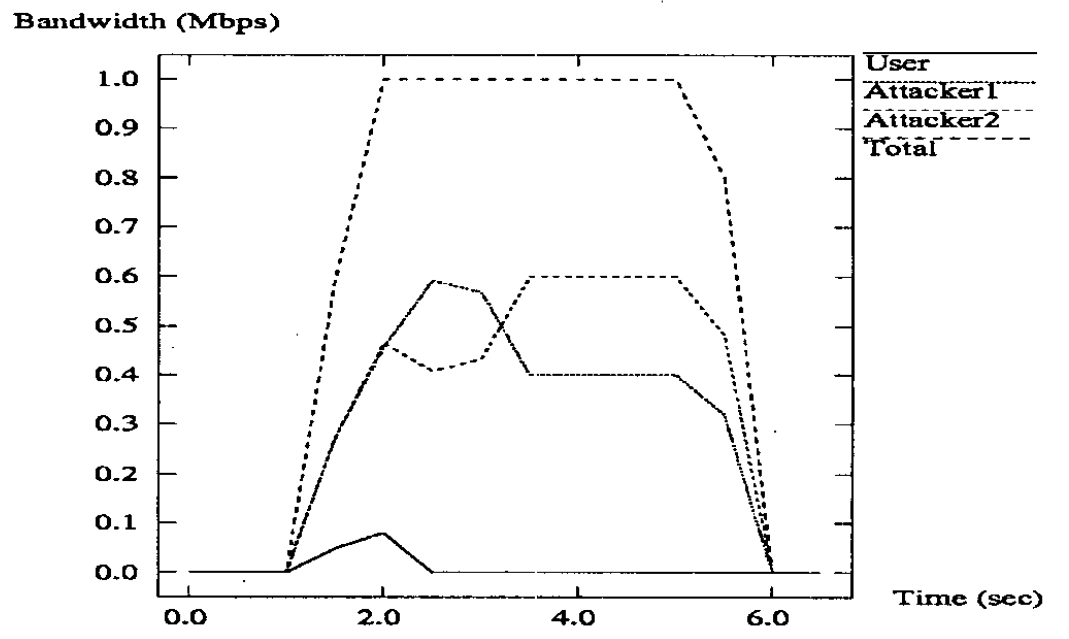
\includegraphics[width=0.45\textwidth]{../Figures/fig4.png} \caption{User's bandwidth during the attack using a DropTail queue \cite{bertsekas1992data}, Figure 4 of \cite{lau2000distributed}.} \label{fig4}
\end{figure}

\begin{figure}[b!]
    \centering
    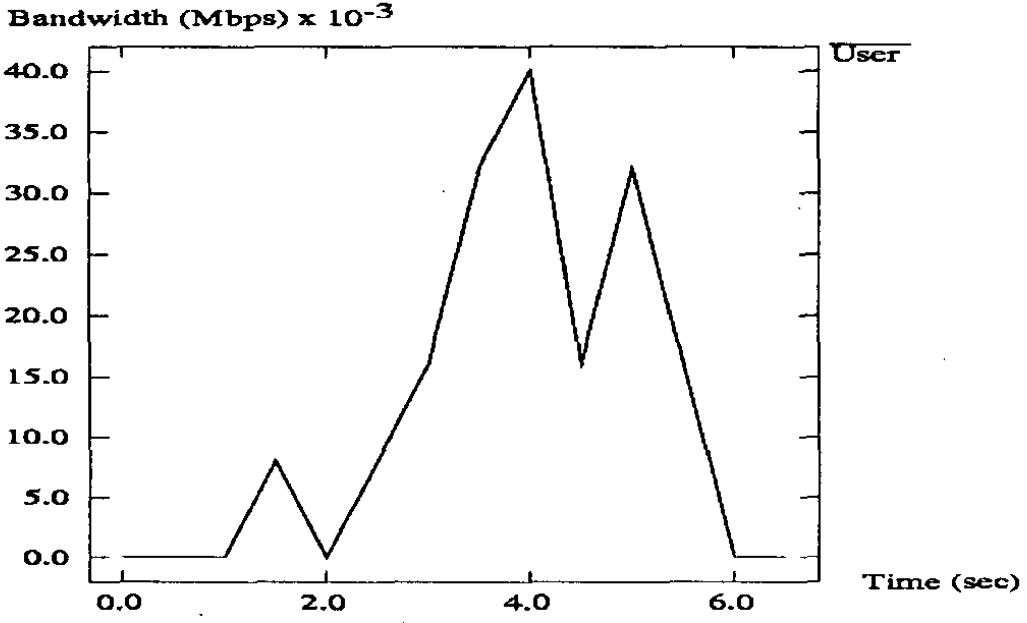
\includegraphics[width=0.45\textwidth]{../Figures/fig5.png} \caption{User's bandwidth during the attack using a RED queue \cite{floyd1993random}, Figure 5 of \cite{lau2000distributed}.} \label{fig5}
\end{figure}

\section{Introduction}

A Denial of Service (DoS) attack is defined as an attempt to make a machine or a resource unavailable to its legitimate users \cite{bellovin1989security}.
When we have more than one source attacing the target, it is called a Distributed DoS (DDoS) \cite{lau2000distributed}.
Typically, attackers try to take control of a lot of unique IP addresses (Zombie Machines) and use them to exhaust a resource either on the target machine, or the network that connects legitimate users to the target machine/s.

%%%%%%%%5add the figure yourself.

\begin{figure}
    \centering
    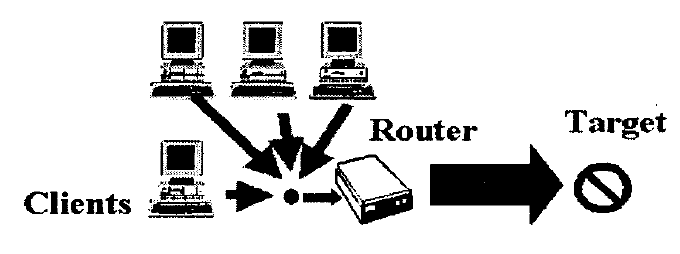
\includegraphics[width=0.35\textwidth]{../Figures/sample.png} \caption{A simple DDoS attack \cite{lau2000distributed}.} \label{sampleDDoS}
\end{figure}

In this experiment, we perform a simple DDoS attack.
As shown in Figure~\ref{sampleDDoS}, a client tries to reach a service through a single hop network with a router connecting it to the server.
Assuming that an attacker takes control of a set of zombie machines connected to the same router, we simulate how he/she can make the service unavailable to the client by targeting the router and overwhelming its queue.
As an outcome, packets will be droped while the attack is in progress and the client will experience a considerable drop in its bandwidth.
Therefore, the key metric in this experiment is the rate at which client communicates with the server while the attack is in progress.
A rate of zero indicates no connectivity and a rate drop indicates service degradation.

\begin{figure}
    \centering
    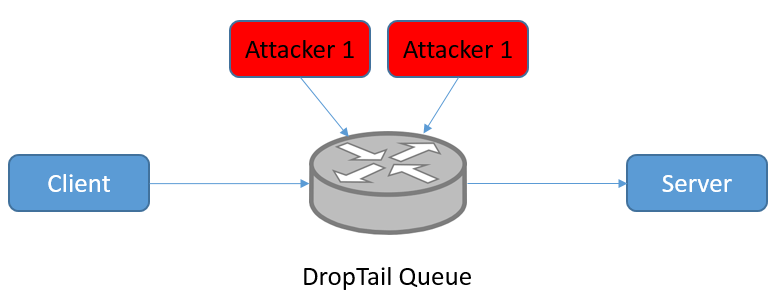
\includegraphics[width=0.5\textwidth]{../Figures/arch1.png} \caption{Architecture for DropTail queue.} \label{arch1}
\end{figure}

\begin{figure}
    \centering
    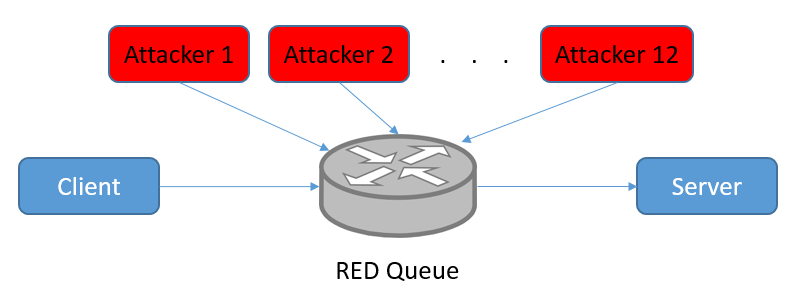
\includegraphics[width=0.5\textwidth]{../Figures/arch2.png} \caption{Architecture for RED queue.} \label{arch2}
\end{figure}

\section {Experiment Design}

Similar to the original experiment, the client establishes a constant bit rate (CBR) UDP stream to the server.
To verify Figure 4, we show that only 2 zombie machines, as in the figure \ref{arch1}, sending CBR traffic are sufficient to disrupt the service when router implements DropTail queueing policy.
Figure 5 shows how queues with Random Early Detection (RED) policy perform under a DDOS attack.
However, in this scenario we need more zombie machines, as in figure \ref{arch2}, to disrupt the service.
Results from the original paper show that unlike DropTail, the client rate will be decreased rather than going down to zero.
It is still considered to be a successful attack as the client experience noticeable service degradation.

Since the authors have not specified the parameters, setting the proper parameters is the toughest part for this project especially for the second part where we experiment with RED, since configuring RED is known to be difficult when it comes to setting proper parameters \cite{floyd1993random}.

\subsection{Choosing the Right Parameters}

For the DropTail queue, we know that the queue rate should be smaller than sum of the clients and two attackers’ rate.
Therefore for NS2 simulation I am sticking to CBR rates 0.1Mbps for client and 0.6Mbps for zombie machines using 500B packets all of which to be aggregated on a queue with rate 1Mbps.
Queue size will also be set to the bandwidth delay product (assuming 1ms RTT): $1Mbps*1ms=1Kb=125B$.
For GENI testbed, we can use tc, where we stick to parameters from lab2 with limited buffer size according to the average RTT of given VMs using bandwidth-delay product (i.e. around 125B per milli second of RTT).

For RED experiment, we have to set 5 parameters: buffer space, $min_{th}$, $max_{th}$, $max_p$, and $w_q$.
RED paper suggests $max_{th}$ to be set at least twice as $min_{th}$, author of RED in answer to another question \cite{red} suggests a value of 3 times as a rule of the thumb.
We will stick to the same ratio in this experiment.
She also suggests a value of 0.1 for $max_p$.
$min_{th}$’s default value in NS2 is 5 packets, for this experiment we set it to 2500B, 5 times our packet size.
$w_q$ should be at least 0.001, NS2 uses 0.002 by default.

To summarize, since parameters are not specified by DDoS paper, my strategy for obtaining the results from RED is to stick to rule of the thumb values suggested by the author as well as NS2 defaults.
If I fail to reproduce results using these values, I will report how and why I changed them to obtain results closer to those of the original paper.

Table \ref{tt} summarizes the parameters for the two experiments.

\begin{table}
    \centering
    \begin{tabularx}{0.5\textwidth}{X|X|X}
        Parameter & DropTail Simulation & RED Simulation \\
        Number of Attackers & 2 & 12 \\
        Total Attack Bandwidth & 1.2Mbps & 9Mbps \\
        Queue Size & 125 B/msRTT & 125 B/msRTT \\
        Client's Desired Rate & 0.1Mbps & 0.1Mbps \\
    \end{tabularx}
    \caption{Related parameters.}\label{tt}
\end{table}

%In addition to reproducing the results, I will also produce a sensitivity analysis by changing the total attack bandwidth and measuring the average user bandwidth and average packet drops.
%Two diagrams will be included in the report: average user bandwidth versus total attack bandwidth and average user packet drops versus total attack bandwidth.

%The original results is a simulation result.
%We will reproduce it using NS2, the same simulation tool, as well as a GENI testbed.

The workload on this experiment, both at the client and zombie machines, consists of synthetic traffic of CBR UDP with packets of 500 bytes.
For the testbed we will produce this traffic using D-ITG.

To conclude the experiment we will analyze the data by computing average client bandwidth and packet drops against variable total rate of attack.
For each factor we plot the mean value of five replications and indicate the range of the mean across replications. 

\section{Results}
\begin{figure}[t!]
    \centering
    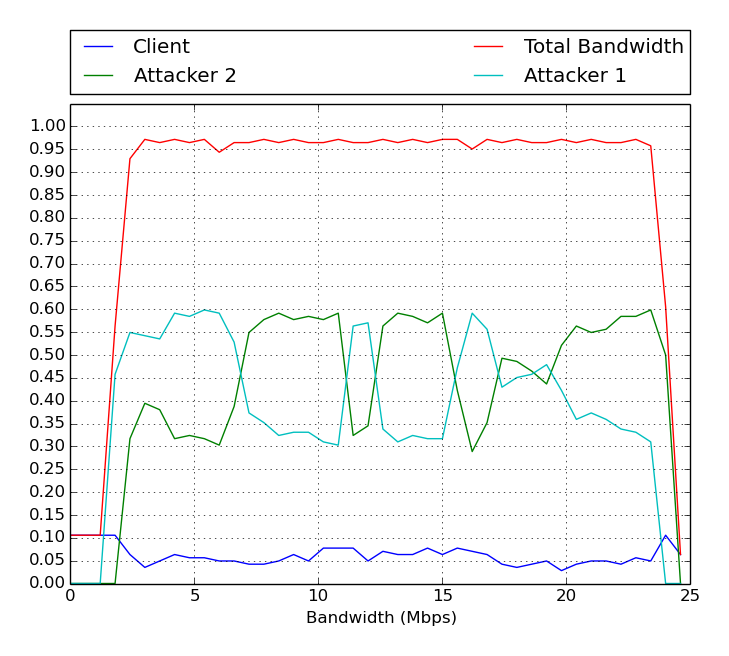
\includegraphics[width=0.5\textwidth]{../Results/tbf.png} \caption{DDOS attack on a DropTail queue.} \label{tbf1}
\end{figure}

\begin{figure}[t!]
    \centering
    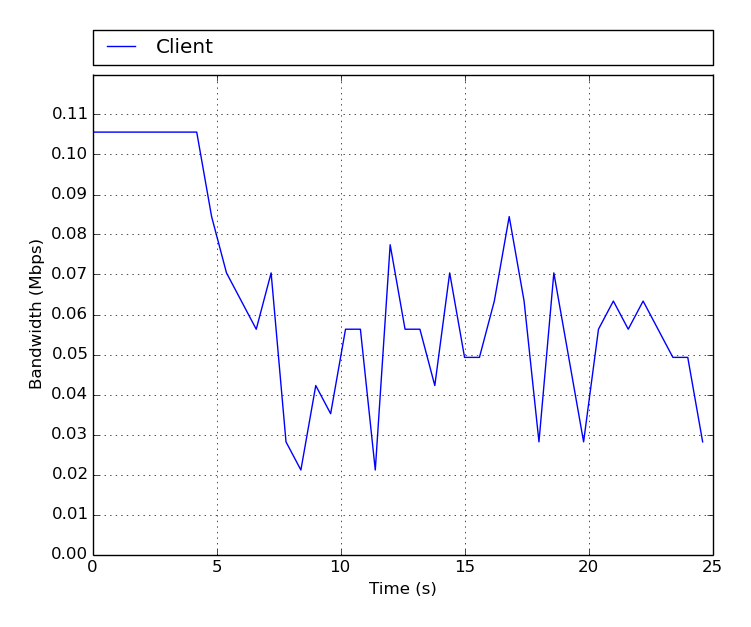
\includegraphics[width=0.5\textwidth]{../Results/red_client.png} \caption{Client bandwidth while RED router is DDOS'ed.} \label{red1}
\end{figure}


\begin{figure}[h!]
    \centering
    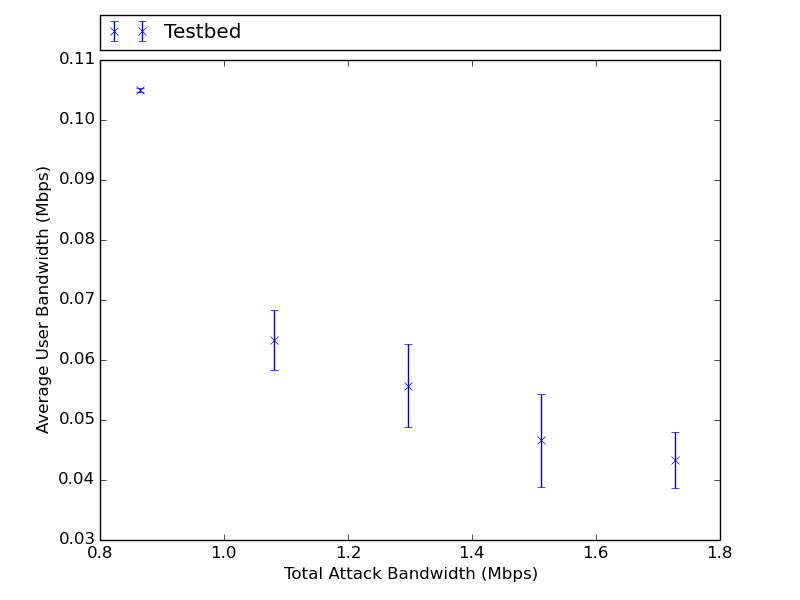
\includegraphics[width=0.5\textwidth]{../Results/result-tbf.png} \caption{Sensivitivity analysis for DropTail queues.} \label{tbf2}
\end{figure}

\begin{figure}[h!]
    \centering
    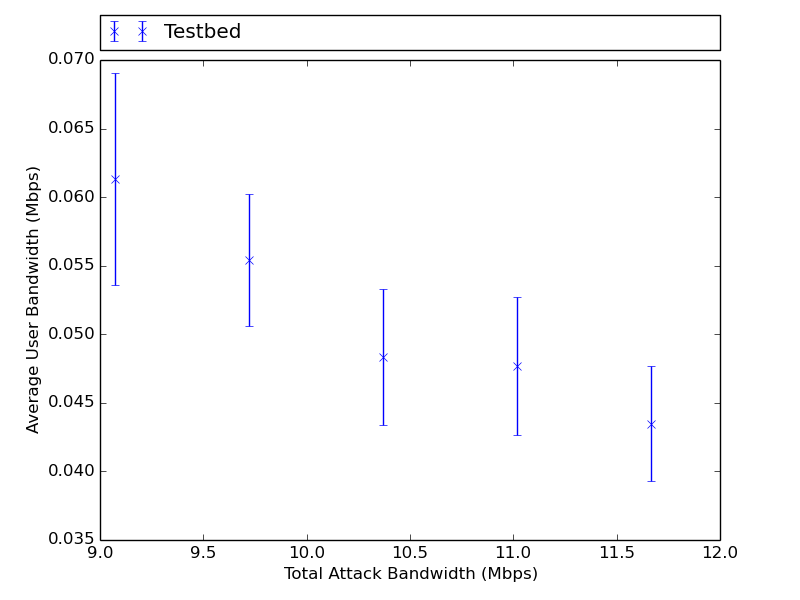
\includegraphics[width=0.5\textwidth]{../Results/result-red.png} \caption{Sensivitivity analysis for RED queues.} \label{red2}
\end{figure}

For Figure 4 of the original paper, I was unable to verify that the client receive no bandwidth.
Instead, the experiment results in Figure~\ref{tbf1} show that the client experiences a noticable rate drop.

For Figure 5 of the orgibal paper, I can verify the result.
The experiment results in Figure~\ref{red1} show that the client maintains connectivity under RED even though attackers flood 9Mbps of packets to the router

Further, I also analysed how sensitive these results are to do change of total attack bandwidth.
As shown in Figure~\ref{tbf2}, under DropTail queue, attackers can further degrade the client's desired rate by flooding more data.

Under RED however, Figure~\ref{red2} shows that increasing total attack bandwidth does not affect the user by a noticable margin:

\bibliographystyle{plain}
\bibliography{ref.bib}

\end{document}
